\section{Data parallel real-time visualisation}

\begin{figure*} [t!]
  \centering
  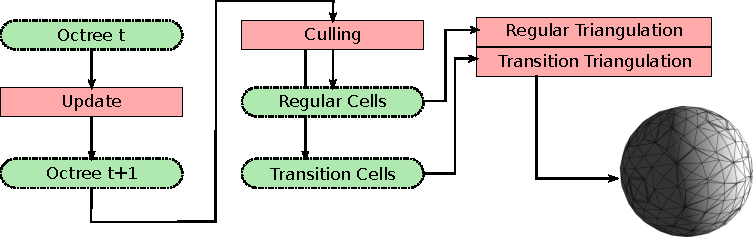
\includegraphics[width=0.9\textwidth]{pipeline}
  \caption{ This figure summarizes our GPU pipeline. Data buffers are represented in green and computations in red. Each computation retrieves data from a buffer and fills a new one. }
  \label{fig_pipeline} 
\end{figure*}

\paragraph{}
We present a new tool for isosurfaces visualisation that is adapted to rasterization issues and runs in real-time.
It is based on the adaptive triangulation of Lengyel \textit{et al}. \cite{lengyel2010voxel}, the linear quadtrees  of Gargantini \cite{gargantini1982effective}, and the LoD criterion of Dupuy \textit{et al.} \cite{dupuy2014quadtrees}.


\paragraph{}
Our pipeline is divided in 3 parts.
\begin{itemize}
\item The first step consists in updating a linear octree that maintains the active front of cells.
\item The second step performs both a culling on the octree cells, and creates the transition cells required for a crack-free MC triangulation.
\item The last step re-subdivides and triangulates the remaining cells.
\end{itemize}
This whole process is illustrated in Figure \ref{fig_pipeline}.
In the following sections, we present each step of our solution.

\subsection{Maintaining the linear octree}

Our method triangulates a set of cells.  Therefore, the first step of
our pipeline evaluates a LoD criterion on each cell to determine if it
is kept, split or merged.  In this section, we present the GPU
representation for those trees, as well as the criterion we use to
evaluate the new partition.

\subsubsection*{Linear octree on the GPU}

\begin{figure}
\centering
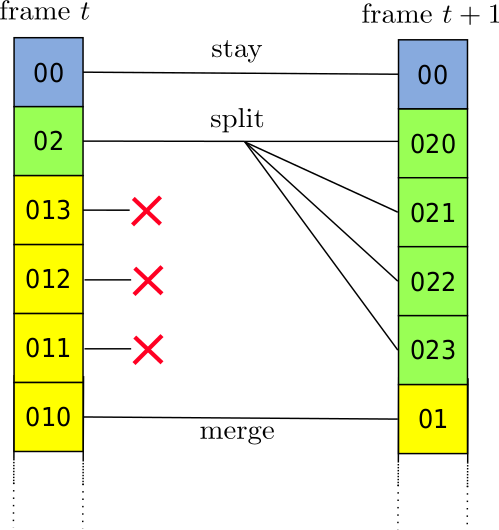
\includegraphics[height=0.2\textheight]{subdivision}
\caption{The octree at frame $t$ is stored as a list of Morton codes in a buffer. 
To update the tree, we fill a new buffer representing its state at frame $t+1$. 
On the GPU, each code of the first buffer is processed in parallel. 
If the cell is to be subdivided, it writes the codes of its children in the new buffer. 
If it merges, it writes either nothing, or the code of its parent (if it is the first child).
If it is kept, it just re-writes its own code. }
\label{subdivision}
\end{figure}

\paragraph{}
Dupuy \textit{et al}. \cite{dupuy2014quadtrees} proposed an implementation to handle efficiently quadtrees on the GPU.
Here, we want to manipulate an octree, hence, we generalize their solution to the third dimension.

\paragraph{}
To represent the cells, we use Morton codes.
Those codes are a succession of locations relatively to the root node.
In three dimensions, there are $2^3 = 8$ possible locations for a node so 3 bits are required to encode one subdivision.
Thus, if we keep the codes on 32 bits as in \cite{dupuy2014quadtrees}, we will be limited to a maximal subdivision depth of 9.
This is too coarse to do a correct triangulation of the surface.
Therefore, we used 64 bits for the encoding. 
This doubles the memory size of the front but, by using 5 bits for the depth of the cell and the other 59 bits for the code, we can subdivide 19 times.

\paragraph{}
At each frame we have the active front of the previous frame, $t$, and we want to update it to get the front at frame $t+1$.
To do so, we evaluate the LoD criterion given in equation (\ref{lod_criterion}) on every cell at frame $t$.
We then test the equations (\ref{split_test}) and (\ref{merge_test}) to determine if the cell should split or merge.
If a cell splits, it emits the codes of its children.
If a cell is kept it re-emits its own code.
If a cell merges, there are two possibilities.
If it is the first child (with the lowest Morton code), it emits the code of its parent.
Otherwise, it does nothing. 
This ensures that the merging operation produce only one cell.
The new cells are written into a new buffer that represents the active front at frame $t+1$.
This is illustrated Figure \ref{subdivision}.

\subsubsection*{Improved LoD criterion}

\paragraph{}
Dupuy \textit{et al.} manipulated quadtrees, a two dimensional structure, which contained a reasonable amount of cells in their active front.
This amount is greater when using an octree as those structures are in three dimensions.
We thus extended the LoD criterion determining the partition to minimize the size of the front.
Note that our extended criterion could still be used in two dimensions.

\paragraph{}
Here, we use the criterion given equation (\ref{lod_criterion}).
Its evaluation is data parallel and controls the projected size of the cells.
However, it is based on the Euclidean distance between a cell and the camera. 
Since this distance is absolute, cells behind the camera are highly subdivided even though they do not contribute to the final image.
Therefore, we combine this Euclidean distance with a radial angle to the camera's forward direction.
Cells behind the camera are then less subdivided, which reduces the number of cells in the octree.
The new criterion is given equation \ref{improved_lod_criterion} and illustrated Figure \ref{fig_lod_octree}.
\\
\begin{equation}
z'= z +
\begin{cases}
    w \cdot z \cdot (\theta - \alpha) 	& \text{if } \theta \geq \alpha\\
    0	              		    			& \text{else.}
\end{cases}
\label{improved_lod_criterion}
\end{equation}

\begin{figure}
  	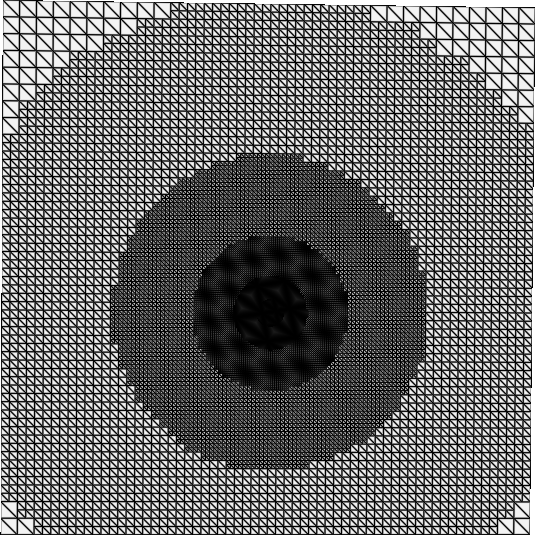
\includegraphics[width=0.4\linewidth]{viewlod1_small}
  	\hfill
  	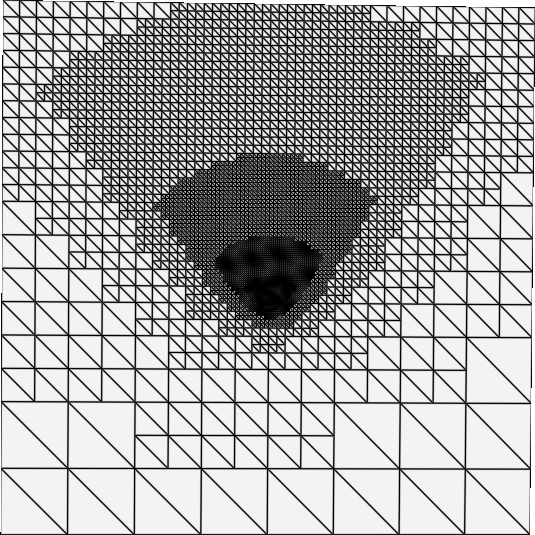
\includegraphics[width=0.4\linewidth]{viewlod2_small}
  \caption{ Adaptive triangulation of a plane. The camera is located in the center and looks up. (Left) uses the criterion in \cite{dupuy2014quadtrees} and (Right) uses our criterion.
  The total number of cells is (Left) 1037114 and (Right) 210323.}
  \label{fig_lod_octree} 
\end{figure}

\paragraph{}
In this equation, $z$ is the Euclidean distance between the center of the cell and the camera, $\theta$ is the angle and $\alpha$ is the fovy, both expressed in radians.
The parameter $w$ controls the importance of the radial distance over the Euclidean distance.
Its value has to be chosen carefully.
If it is too high, the difference of levels between the cells on both side of the frustum becomes very important, which might break the octree consistency. 
Empirically, we found that using $w \leq 6 $ prevents artefacts.

\paragraph{}
With this new $z'$, the criterion evaluated is now $s(z')$ instead of $s(z)$.
Note that we may lose the guarantee of maintaining a restricted octree outside the frustum.
However, as those cells are not triangulated, the visualisation is not impacted.

\subsection{Culling and transitions determination}

\paragraph{}
Once the active front has been updated, it contains the list of the cells to triangulate.
We then apply frustum culling to remove the nodes that are outside the view frustum.
We also remove empty cells; a cell that is fully inside or outside the object will not generate triangles and therefore should not be triangulated.
The remaining cells are stored in a new buffer that is used as input for triangulation.

\paragraph{}
If those cells are directly triangulated, cracks will appear at resolution changes.
As, Lengyel \textit{et al.} \cite{lengyel2010voxel}, we solve this issue by inserting and triangulating transition cells.
At each frame, we identify the level changes in the octree to create the corresponding transitions.
We do so by checking if a cell has a neighbour of higher resolution than itself.
%The difficulty is to do this with a data parallel method.
In our implementation, the chosen LoD criterion is fully data parallel and allows to determine if a cell has been split or merged.
Therefore, we can determine the transitions by evaluating this criterion on the neighbours of a cell.

\paragraph{}
Our LoD criterion is based on the projected size of a cell.
We thus need the position of the neighbours of the current cell.
This is easy to compute as we know the position of the cell and its size.
We then test each of them to determine if it has been split, using equation (\ref{split_test}).
If this test is verified, we emit a transition cell.
Note that each cell can then emit a maximum of 3 transitions, one for each axis.
We finally have two buffers containing the octree and transition cells.

\subsection{Triangulation and further subdivision}

\begin{figure}
  \centering
  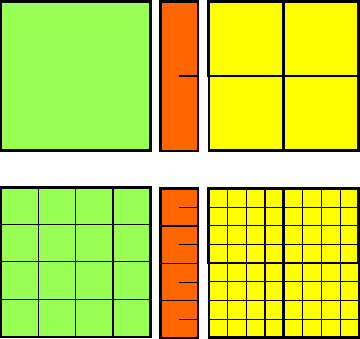
\includegraphics[width=0.6\linewidth]{tessellation}
  \caption{The upper configuration represents a cell with 4 more subdivided neighbours and a transition cell (red).
  This is what is returned by the update and culling steps.
  All those cells are subdivided, leading to the configuration presented on the bottom picture.
  Each cell has become a tile of $(2^N)$ cells on each dimension.
  Except for the transition cells, as their width do not change. }
  \label{tessellation} 
\end{figure}

\paragraph{}
We added a subdivision pass to increase the resolution of the extracted triangulation while staying real-time. 
When triangulating cells that are in the lowest levels of the octree, the resulting mesh is more precise. 
However, with a deeper octree, the update and culling steps are slowed down by the high number of cells to process.
We aim here at keeping the triangulation precise but with a coarser octree.

\paragraph{}
Therefore, a subdivision pass is added between the culling and the triangulation. 
It applies on every octree cell and on every transition cell.
Each octree cell is turned into a regular grid of smaller cells with a resolution of $(2^N)^3$, $N$ being a positive integer controlling the new level of subdivision.
The transition cells have a fixed width so they become a regular grid with a resolution of $(2^N)^2$ (Figure \ref{tessellation}).
This subdivision happens before the triangulation but after the LoD and culling.
This way, those first two steps run on a coarser octree, keeping their efficiency, while the triangulation is done on smaller cells, leading to a more precise mesh.

\paragraph{}
However, no culling is done on the new smaller cells.
Therefore, they will all be triangulated even if they are empty or outside the frustum. 
There is then a $N$ for which it is more interesting to cull a deeper tree than to subdivide the cells. 
Our experiments showed that the best $N$ is 2.

\paragraph{}
The last step is then to apply MC with the modified tables given by Lengyel \textit{et al.} to triangulate the cells and render our surface.
